
O documento de visão tem como objetivo definir uma visão geral do projeto, apresentar os problemas, os requisitos funcionais, não funcionanis, atores entre outras informações que serão definidos com o cliente a fim de garantir que a equipe de desenvolvimento e o cliente estejam na maior sincronia possível \cite{IBM:2014:Online}.

\subsection{Posicionando}
\subsubsection{Oportunidade de Negócios}

Atualmente as ferramentas no mercado possuem limitações, como de qualidade, falta de flexibilidade na gerência, ou até mesmo o fechamento do código, que pode ser considerado uma limitação devida a redução de mão de obra para manutenção e evolução.

\subsubsection{Instrução do Problema}

A \er{} possui diversas \textit{rotas} possíveis para se seguir, como por exemplo a rota ágil, tradicional ou até mesmo uma mistura das duas.

Infelizmente cada ferramenta de gerência de requisitos é voltada para uma dessas possibilidades, tornando díficil a tarefa voltada para outras, gerando assim nos engenheiros de requisitos a necessidade de aprender a utilizar diversas ferramentas para poder organizar projetos com \textit{rotas} diferentes.

A utilização de apenas uma ferramenta que abrangesse as duas metodologias e ainda uma mistura das duas resolveria todo problema de gerência de requisitos em projetos que não se adequam a uma metodologia específica perfeitamente.

\subsubsection{Instrução de Posição do Produto}

Para os engenheiros de \er, a \nomeferramenta representará um avanço nas atividades de gerenciamento, pois os mesmos apenas precisarão aprender as funcionalidades de uma ferramenta, simplificando a mudança entre projetos que tomam rotas distintas.

\subsection{Descrições da Parte Interessada e do Usuário}

Nesta sessão serão identificados e detalhados os interessados e usuários da \nomeferramenta{}.

\subsubsection{Resumo da Parte Interessada}

\begin{itemize}
	\item \textbf{Nome}:
		Engenheiros de software ou qualquer interessado no desenvolvimento de software.
	\item \textbf{Representa}:
		Todos os desenvolvedores de software do mundo que precisam gerenciar requisitos de forma flexivel e prática.
	\item \textbf{Função}:
		Função crítica, já que os mesmos serão os clientes diretos da aplicação, deve-se focar na qualidade da ferramenta para garantir boa aceitação dos mesmos.
\end{itemize}
%Lista todas as partes interessadas identificadas. Para cada tipo de parte interessada, forneça estas informações:
%Nome: Nome do tipo da parte interessada.
%Representa: Descreve brevemente quais pessoas, equipes ou organizações esse tipo de parte interessada representa.
%Função: Descreve brevemente a função que esse tipo de parte interessada desempenha no esforço de desenvolvimento.

\subsubsection{Resumo do Usuário}

	Acho que não se adequa ao documento, voto em retirar este item daqui. Já que nosso usuário é genérico, e por isso, não tem como diferenciá-los.
%Lista todos os tipos de usuários identificados. Para cada tipo de usuário, forneça estas informações:
%Nome: Nome do tipo de usuário
%Descrição: Descreve brevemente o relacionamento desse tipo de usuário com o sistema que está em desenvolvimento.
%Parte Interessada: Lista qual tipo de parte interessada representa esse tipo de usuário.

\subsubsection{Ambiente do Usuário} 
	
	Acho que este item também não se adequa ao documento, pensem aí e me digam o que acham... Por mim eu tiro. Da mesma forma que muitos aí pra baixo... Pensemos até amanhã.
%Detalha o ambiente de trabalho do usuário alvo. Aqui estão algumas sugestões:
%Quantas pessoas estão envolvidas na conclusão da tarefa? Está sendo alterado?
%Quanto tempo leva um loop de tarefa? Quanto tempo os usuários gastam em cada atividade? Está sendo alterado?
%Quais restrições de ambiente exclusivas afetam o projeto? Por exemplo, os usuários requerem dispositivos remotos, trabalham externamente ou trabalham durante as viagens?
%Quais plataformas de sistema estão em uso atualmente? Existem plataformas futuras planejadas?
%Que outros aplicativos estão em uso? Seu aplicativo precisa se integrar a eles?
%Nesta seção, você pode incluir extrações do modelo de negócio para descrever a tarefa e os trabalhadores envolvidos.

\subsubsection{Perfis das Partes Interessadas}
% Descreve cada parte interessada no projeto, preenchendo a seguinte tabela para cada parte interessada. Lembre-se: os tipos de partes interessadas podem ser usuários, departamentos estratégicos, departamentos jurídicos ou de conformidade, desenvolvedores técnicos, equipes de operação, entre outros. Um perfil completo abrange os seguintes tópicos para cada tipo de parte interessada:

%Representante: Determina quem representa a parte interessada para o projeto (Essa informação será opcional se estiver documentada em algum outro lugar.) Insira os nomes dos representantes.
%Descrição: Descreve brevemente o tipo de parte interessada.
%Tipo: Qualifica o conhecimento da parte interessada, como "usuário avançado", "especialista em negócios", ou "usuário informal". Essa designação pode sugerir a experiência técnica e o grau de sofisticação.
%Responsabilidades: Lista as principais responsabilidades da parte interessada no sistema em desenvolvimento; lista seus interesses como uma parte interessada.
%Critérios de Sucesso: Determina como a parte interessada define o sucesso. Como a parte interessada é recompensada?
%Envolvimento - Descreve como a parte interessada está envolvida no projeto. Onde possível, relate o envolvimento nas funções do processo; por exemplo, uma parte interessada pode ser um revisor de requisitos.
%Entregas: Identifica as entregas adicionais que a parte interessada requer. Esses itens podem ser entregas do projeto ou saída a partir do sistema em desenvolvimento.
%Comentários ou Problemas: Determina os problemas que interferem com o sucesso e quaisquer outras informações relevantes.

\subsubsection{Perfis do Usuário}
% Descreve cada usuário do sistema aqui, preenchendo a seguinte tabela para cada tipo de usuário. Lembre-se que os tipos de usuário podem ser especialistas e novatos; por exemplo, um especialista pode precisar de uma ferramenta sofisticada e flexível com suporte para várias plataformas, enquanto um novato pode precisar de uma ferramenta que seja fácil de usar. Um perfil completo abrange esses tópicos para cada tipo de usuário:
%Representante: Indica quem representa o usuário para o projeto. (Essa informação será opcional se estiver documentada em algum outro lugar.) Esse representante, geralmente refere-se à parte interessada que representa o conjunto de usuários; por exemplo, Parte Interessada: Parte Interessada1.
%Descrição: Descreve brevemente o tipo de usuário.
%Tipo: Qualifica o conhecimento do usuário, como "usuário avançado" ou "usuário informal." Essa designação pode sugerir a experiência técnica e o grau de sofisticação.
%Responsabilidades: Lista as principais responsabilidades do usuário com respeito ao sistema; por exemplo, determina quem captura os detalhes do cliente, produz relatórios e coordena trabalho, etc.
%Critérios de Sucesso: Determina como o usuário define o sucesso. Como o usuário é recompensado?
%Envolvimento: Descreve como o usuário está envolvido no projeto. Onde possível, relate o envolvimento nas funções do processo; por exemplo, uma parte interessada pode ser um revisor de requisitos.
%Entregas: Identifica as entregas que o usuário produz e para quem.
%Comentários ou Problemas: Determina os problemas que interferem com o sucesso e quaisquer outras informações relevantes. Descreve as tendências que tornam a tarefa do usuário mais fácil ou mais difícil.

\subsubsection{Principais Problemas e Necessidades da Parte Interessada}

O problema a ser atacado pela solução de software deve estar bastante claro entre todos os \textit{stakeholders} para que o desenvolvimento da ferramenta não passe por nenhuma dificuldade quanto ao entendimento de onde focar para realizar a solução do problema.

Para o entendimento do problema principal, foi utilizada a técnica de \textit{fishbone}. Segue o resultado da mesma na figura abaixo:

%-------------------------------------FISHBONE AQUI----------------------------------------
\begin{figure}[!h]
	\centering
	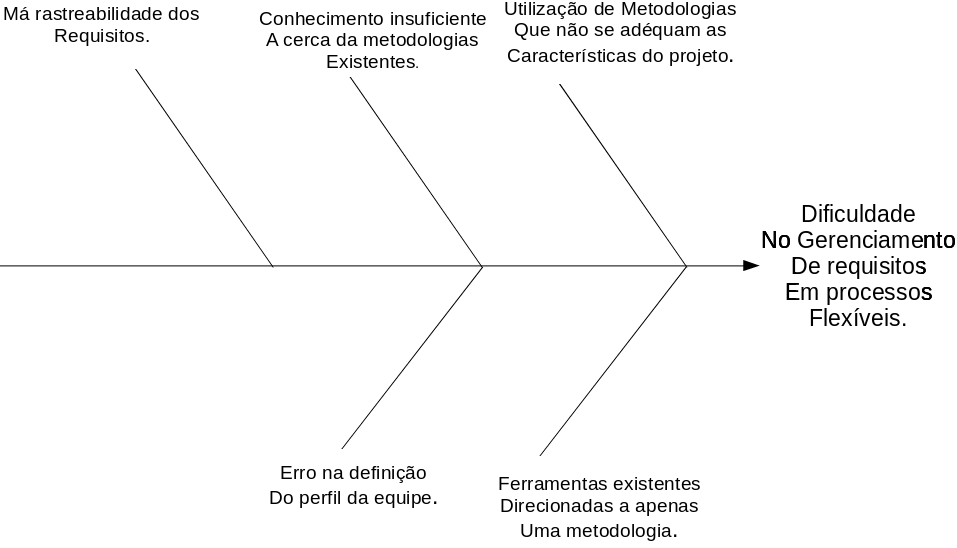
\includegraphics[width=0.8\textwidth]{conteudo/fishbone}
	\caption{Fishbone de Problema}
\end{figure}

Para melhor entendimento do problema, utilizamos a técnica de \textit{Framework de Problema}, na qual apresentamos o problema, os afetados, o impacto do problema e qual seria uma solução bem sucedida. Segue o \textit{framework de Problema}:

\begin{table}[htbp]
\centering
\begin{tabular}{|p{2.5cm}|p{10cm}|p{2.5cm}|}
\hline
\textbf{O Problema:} & Dificuldade no Gerenciamento de requisitos em processos flexíveis. \\ \hline
\textbf{Afeta:} & Todos os desenvolvedores de software que necessitam de uma flexibilidade maior na gerência de requisitos. \\ \hline
\textbf{Cujo impacto é:} & Software mal desenvolvidos, proporcionando maior possibilidade de erros. \\ \hline
\textbf{Uma solução bem sucedida seria:} & Utilização de uma ferramenta que faça gerência de requisitos de forma flexivel, podendo utilizá-la em qualquer metodologia. \\ \hline
% Ambiente & Preparar  Estrutura de documentos e diretórios para geração de relatórios & Luiz Oliveira \\ \hline
\end{tabular}
\label{}
\caption{Framework de Problema}
\end{table}

Após o entendimento do problema, vê-se necessária a documentação das necessidades do cliente, para mesma, utilizou-se de uma técnica chama \textit{framework de necessidades} na qual são apresentados todos os problemas, as necessidades, a solução atual e a solução proposta. Dessa forma, pode-se obter um entendimento mais organizado dos problemas e necessidades do cliente. Segue o \textit{framework de necessidades}:

\begin{table}[htbp]
\centering
\begin{tabular}{|p{5cm}|p{3cm}|p{3cm}|p{5cm}|}
\hline
\textbf{Necessidade} & \textbf{Problema} & \textbf{Solução Atual} & \textbf{Solução Proposta}  \\ \hline

Obter uma opinião da melhor metodologia a ser seguida de acordo com as características do projeto. & Utilização de metodologias que não se adéquam as características do projeto. & A equipe de desenvolvimento escolhe a sua metodologia. & Criação de uma ferramenta que apresente a melhor opção de metodologia a ser seguida, de acordo com as características do projeto.\\ \hline

Obter a metologia que melhor se adequa ao contexto, mesmo sem ter conhecimento profundo sobre a mesma. & onhecimento insuficiente a cerca das metodologias existentes. & Estudar as metodologias existentes. & Criação de uma ferramenta que faça a seleção da melhor metodologia sem que os envolvidos precisem ter conhecimento sobre a mesma. \\ \hline

Criação de uma rastreabilidade de fácil entendimento e bem organizada. & Má rastreabilidade dos requisitos. & Realizar a rastreabilidade a partir do conhecimento da equipe. & Utilização de uma ferramenta que documente os requisitos tomando cuidado com a rastreabilidade do mesmo, garantindo organização e fácil entendimento. \\ \hline

Necessidade de ferramentas flexíveis, que utilizam determinada metodologia de acordo com as características do projeto. & Ferramentas existentes direcionadas a apenas uma metodologia. & Utilização de mais de uma ferramenta. 4 & Criação de uma ferramenta que utilize todas as metodologias, se adequando as características do projeto. \\ \hline

Obter o perfil da equipe já definido. & Erro na definição do perfil da equipe. & A própria equipe define seu perfil. & Criação de uma ferramenta que apresente o perfil da equipe a partir de \textit{inputs} que representam algumas características da mesma. \\ \hline

\end{tabular}
\label{}
\caption{Framework de Necessidades}
\end{table}
%Lista os principais problemas com soluções existentes como observadas pela parte interessada. Esclarece estas questões para cada problema:
%Quais são os motivos para esse problema?
%Como o problema é resolvido agora?
%Quais soluções a parte interessada deseja?
%Você deve entender a importância relativa que a parte interessada coloca na solução de cada problema. A classificação e técnicas de votos acumulativos indicam os problemas que devem ser resolvidos versus os problemas que as partes interessadas gostariam de tratar. Use esta tabela para capturar as necessidades da parte interessada.
%Tabela 1. Necessidades da Parte Interessada
%Necessidade	Prioridade	Interesses	Solução atual	Solução proposta
 	 	 	 	 
\subsubsection{Alternativas e Concorrência}
%Identifica as alternativas que a parte interessada percebe como disponíveis. Essas alternativas podem incluir a compra do produto de um concorrente, a criação de uma solução desenvolvida internamente ou manter o status quo. Listam todas as opções disponíveis e conhecidas. Elas incluem os principais pontos fortes e fracos de cada concorrente como observados pela parte interessada.

\subsection{Visão Geral do Produto}
%Esta seção fornece uma visualização de alto nível das capacidades do produto, interfaces para outros aplicativos e configurações dos sistemas. Esta seção, em geral, consiste em três subseções:
%Perspectiva do Produto
%Funções do Produto
%Suposições e Dependências

\subsubsection{Perspectiva do Produto}
%Coloca o produto em perspectiva com respeito a outros produtos relacionados e ao ambiente do usuário. Se o produto for independente e totalmente autocontido, indique-o aqui. Se o produto for um componente de um sistema maior, relacione como esses sistemas interagem e identificam as interfaces relevantes entre os sistemas. Uma maneira de exibir os principais componentes do maior sistema, interconexões e interfaces externas é usar um processo de negócios ou diagrama de casos de uso.

\subsubsection{Resumo das Capacidades}
%Resume os principais benefícios e recursos que o produto fornecerá. Por exemplo, um sistema de suporte ao cliente pode usar essa parte para endereçar a documentação do problema, o roteamento e o relato de status sem elaborar em detalhes o que essas funções requerem. Organize as funções de modo que a lista seja compreensível para o cliente ou para qualquer outra pessoa que leia o documento pela primeira vez. Uma simples tabela que lista os principais benefícios cujos recursos de suporte são suficientes, como no exemplo a seguir.
%Tabela 2. Exemplo de Benefícios e Recursos
%Benefício para o Cliente	Recursos de Suporte
%A nova equipe de suporte pode aprender rapidamente como usar o produto.	A base de conhecimento ajuda a equipe de suporte a identificar rapidamente as correções e soluções alternativas conhecidas.
%A satisfação do cliente é melhorada porque não há falhas.	Os problemas são exclusivamente detalhados em itens, classificados e controlados em todo o processo de resolução. A notificação automática ocorre para quaisquer problemas anteriores.
%O gerenciamento pode identificar as áreas com problema e calibrar a carga de trabalho da equipe.	Os relatórios de tendência e distribuição permitem a revisão de alto nível do status do problema.
%Equipes de suporte distribuídas podem trabalhar juntas para resolver problemas.	Com um servidor de replicação, as informações do banco de dados podem ser compartilhadas em toda a empresa.
%Os clientes podem se ajudar, reduzindo os custos de suporte e melhorando o tempo de resposta.	A base de conhecimento pode ficar disponível na Internet. A base de conhecimento inclui recursos de pesquisa de hipertexto e um mecanismo de consulta gráfica.

\subsubsection{Suposições e Dependências}
%Lista cada um dos fatores que afeta os recursos que o documento de visão inclui. Lista as suposições que, se modificadas, alterarão o documento de visão. Por exemplo, uma suposição pode indicar que um sistema operacional específico fique disponível para o hardware designado para o produto de software. Se o sistema operacional não estiver disponível, será necessário alterar o documento de visão.

\subsubsection{Licenciamento e Instalação}
%Os problemas de licenciamento e instalação também podem impactar diretamente o esforço de desenvolvimento. Por exemplo, a necessidade de suportar a serialização, a segurança da senha ou o licenciamento da rede criarão requisitos adicionais do sistema que devem ser considerados no esforço de desenvolvimento. Os requisitos de instalação também podem afetar a codificação ou criar a necessidade de separar o software de instalação.

\subsection{Recursos do Produto}
%Lista e descreve brevemente os recursos do produto. Os recursos são capacidades de alto nível do sistema que são necessários para entregar benefícios aos usuários. Cada recurso é um serviço solicitado que, em geral, requer uma série de entradas para alcançar o resultado desejado. Por exemplo, um recurso de um sistema de rastreamento de problemas pode ser a capacidade de fornecer relatórios de tendências. À medida que o modelo de casos de uso toma forma, atualize a descrição para fazer referência aos casos de uso.

%Como o documento de visão é revisado por uma ampla variedade de equipes envolvidas, mantenha o nível de detalhes gerais suficiente para que todos possam entender. No entanto, ofereça detalhes suficientes para fornecer à equipe as informações que ela precisa para criar um modelo de casos de uso ou outros documentos de design.

%Para gerenciar a complexidade do aplicativo, para um novo sistema ou uma mudança incremental, liste os recursos em um alto nível para que você possa incluir aproximadamente 25 a 99 recursos. Esses recursos fornecem a base para a definição do produto, gerenciamento de escopo e gerenciamento do projeto. Cada recurso será expandido mais detalhadamente no modelo de casos de uso.

%Em toda esta seção, torne cada recurso relevante para usuários, operadores ou outros sistemas externos. Inclua uma descrição de funções e problemas de usabilidade que devem ser tratados. As seguintes diretrizes se aplicam:
%Evite design. Mantenha as descrições do recurso em um nível geral. Foque nas capacidades necessárias e por que (não como) elas devem ser implementadas.
%Designe todos os recursos como requisitos de um tipo de recurso específico para fácil referência e rastreamento.

\subsubsection{Recurso 1}

\subsubsection{Recurso 2}

\subsection{Restrições}
%Observe todas as restrições de design, restrições externas, como requisitos operacionais ou regulamentares) ou outras dependências.

\subsection{Faixas de Qualidade}
%Defina as faixas de qualidade para desempenho, robustez, tolerância a falhas, usabilidade e características similares que o conjunto de recursos não descreve.

\subsection{Precedência e Prioridade}
%Define a prioridade dos diferentes recursos do sistema.

\subsection{Outros Requisitos do Produto}
%Em um alto nível, lista os padrões aplicáveis, os requisitos de hardware ou plataforma, os requisitos de desempenho e os requisitos ambientais.

\subsubsection{Padrões Aplicáveis}
%Lista todos os padrões que o produto deve estar em conformidade. A lista pode incluir estes padrões:
%Padrões jurídicos e regulamentares (FDA, UCC)
%Padrões de comunicações (TCP/IP, ISDN)
%Padrões de conformidade da plataforma (Windows, UNIX, etc.)
%Padrões de qualidade e segurança (UL, ISO, CMM)

\subsubsection{Requisitos do Sistema}
%Define os requisitos do sistema para o aplicativo. Eles incluem os sistemas operacionais do host suportados e as plataformas de rede, configurações, memória, dispositivos periféricos e software de parceiros.

\subsubsection{Requisitos de Desempenho}
%Detalha os requisitos de desempenho. Os problemas de desempenho podem incluir itens como fatores de carga do usuário, largura de banda ou capacidade de comunicação, rendimento, exatidão, confiabilidade ou tempos de resposta em uma variedade de condições de carregamento.

\subsubsection{Requisitos Ambientais}
%Detalha os requisitos ambientais conforme necessário. Para sistemas baseados em hardware, os problemas ambientais podem incluir temperatura, choque elétrico, umidade e radiação. Para aplicativos de software, os fatores ambientais podem incluir condições de uso, ambiente do usuário, disponibilidade do recurso, problemas de manutenção, manipulação de erros e recuperação.

\subsection{Requisitos de Documentação}
%Esta seção descreve a documentação que deve ser desenvolvida para suportar a implementação bem sucedida do aplicativo.

\subsubsection{	Notas sobre a liberação, arquivo Leia-me}
%As notas sobre a liberação ou um arquivo Leia-me abreviado podem incluir uma seção "O que Há de Novo", uma discussão sobre problemas de compatibilidade com liberações anteriores, e alertas de instalação e atualização. O documento pode também conter ou vincular correções na liberação e quaisquer problemas ou soluções alternativas conhecidos.

\subsubsection{Ajuda On-line}
%Muitos aplicativos fornecem um sistema de ajuda on-line para ajudar o usuário. A natureza desses sistemas é exclusiva para desenvolvimento de aplicativo, pois eles combinam aspectos de programação (centros de informações pesquisáveis e navegação do tipo Web) com aspectos de composição técnica (organização, apresentação). Muitas equipes consideram que o desenvolvimento do sistema de ajuda on-line é um projeto dentro de um projeto que se beneficia do gerenciamento de escopo e planejamento no início do projeto.

\subsubsection{Guias de Instalação}
%Um documento que inclui instalação, configuração e instruções de atualização como parte da oferta de solução integral.

\subsection{Atributos do Recurso}
%Fornece aos recursos atributos que podem ser usados para avaliar, controlar, priorizar e gerenciar os itens de produtos propostos para implementação. Descreve todos os tipos de requisitos e atributos em um plano de gerenciamento de requisitos. No entanto, você pode listar e descrever brevemente os atributos para os recursos que foram escolhidos. As subseções a seguir representam um conjunto de atributos de recursos sugeridos.

\subsubsection{Status}
%Aqui inserir a tabela que esta no doucmento antigo.

\subsubsection{Prioridade}

\subsubsection{Arquitetura}